\documentclass[10pt,oneside]{article}

\usepackage{amsmath}
\usepackage{bm}
\usepackage{mathpazo}
\usepackage{graphicx}
\usepackage{enumerate}
\usepackage[x11names, svgnames]{xcolor} % for \definecolor

\usepackage[letterpaper]{geometry}
\geometry{verbose,tmargin=0.25in,bmargin=0.5in,lmargin=1in,rmargin=1.15in}

 \definecolor{saitPurple}{RGB}{112,40,119}
 \definecolor{statsMaroon}{rgb}{0.55, 0, 0}
 \definecolor{saitMaroon}{rgb}{0.55, 0, 0}
 \definecolor{statsRed}{RGB}{224,38,37}
 \definecolor{saitRed}{RGB}{224,38,37}
 \definecolor{saitBlue}{rgb}{0, 0.59, 0.85}
 \definecolor{statsBlue}{rgb}{0, 0.59, 0.85}
 \definecolor{statsDeepBlue}{RGB}{0, 99, 167}
 \definecolor{saitDeepBlue}{RGB}{0, 99, 167}
 \definecolor{saitDeepBlue}{RGB}{0, 99, 167}
 \definecolor{LightGrey}{RGB}{200,200,200}
%  \definecolor{boxBG}{RGB}{236, 227, 227}
%  \definecolor{boxBG}{RGB}{242, 233, 223}
\usepackage{xcolor}
\usepackage{cancel}
\usepackage{bm}
\usepackage{graphicx}
\usepackage[x11names, svgnames]{xcolor} % for colors in handouts, auto loaded in Beamer?
\usepackage{tikz}
\usetikzlibrary{arrows.meta, math, calc, shadows}
\usetikzlibrary{decorations.markings, decorations.fractals, decorations.text} % for chain, etc.
\usetikzlibrary{intersections}
\usepackage{pgfmath}
\usepackage{ifthen}
\usepgfmodule{oo}
\usepgflibrary{shadings}
% \usetikzlibrary{decorations.shapes}
\usepackage[many]{tcolorbox}
\usepackage[absolute,overlay,showboxes]{textpos}
% \usepackage{textpos}
% \textblockorigin{0.0cm}{0.0cm}  %start all at upper left corner
\TPshowboxesfalse

\newcommand\lb{\linebreak}
\newcommand\Ra{\Rightarrow}
\newcommand\cd{\!\cdot\!}
\newcommand\x{\!\times\!}
\newcommand\pars{\par\smallskip}
\newcommand\parm{\par\medskip}
\newcommand\parb{\par\bigskip}
\renewcommand{\deg}{^\circ}

% counter for resuming enumerated list numbers
\newcounter{resumeenumi}
\newcommand{\suspend}{\setcounter{resumeenumi}{\theenumi}}
\newcommand{\resume}{\setcounter{enumi}{\theresumeenumi}}



% https://tex.stackexchange.com/questions/33703/extract-x-y-coordinate-of-an-arbitrary-point-in-tikz
\makeatletter
\providecommand{\gettikzxy}[3]{%
	\tikz@scan@one@point\pgfutil@firstofone#1\relax
	\edef#2{\the\pgf@x}%
	\edef#3{\the\pgf@y}%
}
\makeatother

\makeatletter
\newcommand{\verbatimfont}[1]{\def\verbatim@font{#1}}%
\makeatother

%%%%%%%%%%%%%%%%%%%%%%%%%%%%%%%%%%%%%%%%%%%%%%%%%%%%%%%%%%%%%%%%%%%%%%%%%%%%%%%%


\newcommand{\tb}[4][0.8]{
	\begin{textblock*}{#1}(#2, #3)
		% \raggedright
		#4
	\end{textblock*}
}

\newtcolorbox{statsbox}[2][] { 
  colback=white,
  colbacktitle=structure,
  colframe=structure,
  coltitle=white,  
  top=0.25cm,
	bottom=0.125cm,
	left=0mm,
	right=0mm,
  % fonttitle=\itshape\rmfamily,
  halign=flush left, 
  enhanced,
  drop fuzzy shadow,
  attach boxed title to top left={xshift=3.5mm, yshift=-2mm},
  title={#2}, #1}
\newtcolorbox{redbox}{colback=white, colframe=structure, enhanced, drop fuzzy shadow}
\newtcolorbox{titledbox}[1]{colback=white,colframe=structure,title={#1}}
\newtcbox{\tcb}[1][]{colback=white,boxsep=0pt,top=5pt,bottom=5pt,left=5pt,
		right=5pt, colframe=structure,  enhanced, drop fuzzy shadow, #1}
% tcb title
\newtcbox{\tcbt}[2][]{colback=white,boxsep=0pt,top=5pt,bottom=5pt,left=5pt,
		right=5pt, colframe=structure, enhanced, drop fuzzy shadow,  title={#2}, #1}
% tcb left title
\newtcbox{\tcbtl}[2][]{ colback=white,
  colbacktitle=structure,
  colframe=structure,
  coltitle=white,  
  top=0.25cm,
	bottom=0.125cm,
	left=0mm,
	right=0mm,
  % fonttitle=\bfseries,
  halign=flush left, 
  enhanced,
  drop fuzzy shadow,
  attach boxed title to top left={xshift=3.5mm, yshift=-2mm}, 
	title={#2}, #1}

\newtcbtheorem{myexam}{Example}%
{
	enhanced,
	colback=white,
	colframe=structure,
	% fonttitle=\bfseries,
	fonttitle=\itshape\rmfamily,
	drop fuzzy shadow,
	%description font=\mdseries\itshape,
	attach boxed title to top left={yshift=-2mm, xshift=5mm},
	colbacktitle=structure
	}{exam}% then \pageref{exer:theoexample} references the theo

% \newcommand{\myexample}[2][red]{
% 	% \tcb\tcbset{theostyle/.style={colframe=red,colbacktitle=yellow}}
% 	\begin{myexam}{}{}
% 		#2
% 	\end{myexam}
% 	% \tcbset{colframe=structure,colbacktitle=structure}
% }

\newtcbtheorem{myexer}{Exercise}%
{
	enhanced,
	colback=white,
	colframe=structure,
	% fonttitle=\bfseries,
	drop fuzzy shadow,
	fonttitle=\itshape\rmfamily,
	% description font=\mdseries\itshape,
	attach boxed title to top left={yshift=-2mm, xshift=5mm},
	colbacktitle=structure
	}{exer}



\newcommand{\mini}[2][0.8]{
	\begin{minipage}[c]{#1\columnwidth}
		\raggedright
		#2
	\end{minipage}
}
\newcommand{\minit}[2][0.8]{
	\begin{minipage}[t]{#1\columnwidth}
		% \raggedright
		#2
	\end{minipage}
}

% centered minipage with text \raggedright
%\cmini[width]{content}
\newcommand{\cmini}[2][0.8]{
	\begin{center}
		\begin{minipage}{#1\columnwidth}
			\raggedright
			#2
		\end{minipage}
	\end{center}
}



\newcommand{\fig}[2][1]{% scaled graphic
	\includegraphics[scale=#1]{#2}
}

% centred framed colored box black border
%\cbox[width]{content}
\newcommand{\cbox}[2][1]{% framed centered color box
	\setlength\fboxsep{5mm}
	\setlength\fboxrule{.2 mm}
	\begin{center}
		\fcolorbox{black}{white}{
			\vspace{-0.5cm}
			\begin{minipage}{#1\columnwidth}
				\raggedright
				#2
			\end{minipage}
		}
	\end{center}
	\setlength\fboxsep{0cm}
}

\newcommand{\cfig}[2][1]{% centred, scaled graphic
	\begin{center}
		\includegraphics[scale=#1]{#2}
	\end{center}
}






% !TEX root = ../Beamer/statikz/statikz.tex

% \Channel[rotate=0]{coordinate}{draw}{fill}{scale}{lineWidth}
\newcommand{\Channel}[6][0]{
	\def\rotate{#1};
	\def\mid{#2}
	\def\lfill{#3}
	\def\lstroke{#4}
	\def\scale{#5};
	\def\lineWidth{#6};

	\begin{scope}[rounded corners=1pt, scale=\scale, rotate=\rotate]
		\filldraw[draw=\lstroke, fill=\lfill, line width=\lineWidth pt] ($(\mid) + (0,-3) $) -- ++(1.7,0) arc(0:85:0.25) -- ($ (\mid)+(0.4,-2.6) $) -- ($ (\mid)+(0.4,2.6) $) -- +(8.13:1.097)arc(-81.87:0:0.25) -- ($ (\mid)+(0,3) $)  -- cycle;
	\end{scope}
}

%\Member{startpt}{endpt}{outer fill color}{inner fill color}{stroke}{height}{radius}{linewidth}
\providecommand{\Member}[8]{
  % name the points
  \coordinate(start) at (#1);
  \coordinate(end) at (#2);
  \edef\ofill{#3}%
  \edef\ifill{#4}%
  \edef\stroke{#5}%
  \edef\height{#6} % cm
  \edef\radius{#7} % cm
  \edef\linewidth{#8} % mm

  \coordinate(delta) at ($ (end)-(start) $);
  \gettikzxy{(delta)}{\dx}{\dy}
  \gettikzxy{(start)}{\sx}{\sy}
  \pgfmathparse{veclen(\dx, \dy)} \let\length\pgfmathresult

  \pgfmathparse{\dx==0}%
  % \ifnum low-level TeX for integers
  \ifnum\pgfmathresult=1 % \dx == 0
    \pgfmathsetmacro{\rot}{\dy > 0 ? 90 : -90}
  \else
    \pgfmathsetmacro{\rot}{\dx > 0 ? atan(\dy / \dx) : 180 + atan(\dy / \dx)}
  \fi

  
   
  \shadedraw[transform canvas = { rotate around = {\rot:(\sx,\sy)}}, line width = \linewidth, rounded corners = \radius mm, top color = \ofill, bottom color = \ofill, middle color = \ifill, draw = \stroke] ($ (start)+(-0.5*\height, 0.5*\height) $) -- ++(\height cm +\length pt, 0 ) -- ++(0, -\height) -- ++ (-\height cm -\length pt, 0) -- cycle;


  \shadedraw[ball color = \ofill!50!\ifill, draw = \stroke] (start) circle (\height/8);
  \shadedraw[ball color = \ofill!50!\ifill, draw = \stroke] (end) circle (\height/8);
  %  \pgfresetboundingbox

  
  


}

%\Member{startpt}{endpt}{outer fill color}{inner fill color}{stroke}{height}{radius}{linewidth}
\providecommand{\Meme}[8]{
  \coordinate(start) at (#1);
  \coordinate(end) at (#2);
  \edef\ofill{#3}%
  \edef\ifill{#4}%
  \edef\stroke{#5}%
  \edef\height{#6} % cm
  \edef\radius{#7} % cm, should be half \height or less
  \edef\linewidth{#8} % mm

  


  \coordinate(delta) at ($ (end)-(start) $);
  \gettikzxy{(delta)}{\dx}{\dy}
  \gettikzxy{(start)}{\sx}{\sy}
  \gettikzxy{(end)}{\ex}{\ey}
  \pgfmathparse{veclen(\dx, \dy)} \let\length\pgfmathresult
  \pgfmathparse{\height*28.435} \let\heightpt\pgfmathresult
  \pgfmathparse{\heightpt/\length} \let\ratio\pgfmathresult
  \pgfmathparse{1/\ratio} \let\inverse\pgfmathresult
  

  \pgfmathparse{\dx==0}%
  % \ifnum low-level TeX for integers
  \ifnum\pgfmathresult=1 % \dx == 0
    \pgfmathsetmacro{\rot}{\dy > 0 ? 90 : -90}
  \else
    \pgfmathsetmacro{\rot}{\dx > 0 ? atan(\dy / \dx) : 180 + atan(\dy / \dx)}
  \fi

  \pgfmathparse{round(mod(abs(\rot),90))} \let\tmp\pgfmathresult
  \pgfmathsetmacro{\rotmod}{\tmp>45?90-\tmp:\tmp}
  \pgfmathparse{(0.007*\rotmod-0.315)/45+1.017} \let\rotfudge\pgfmathresult
  \pgfmathparse{1+3.62/(1+(\inverse/0.714)^1.69)} \let\fudge\pgfmathresult
  \pgfmathparse{50*(1-\ratio)*\fudge*\rotfudge} \let\colorstop\pgfmathresult
  \pgfmathparse{(100-\colorstop)} \let\colorstoptwo\pgfmathresult

  \pgfdeclareverticalshading{myshade}{100bp}{%
					color(0bp)=(\ofill);
					color(\colorstop bp)=(\ofill);
					color(50 bp)=(\ifill);
					color(\colorstoptwo bp)=(\ofill);
					color(100bp)=(\ofill)}

  \begin{scope}[rotate around = {\rot:(start)}, rounded corners = \radius cm, shading angle=\rot]
    \begin{scope} 
      \path[clip]($ (start)+(-0.5*\height, 0.5*\height cm) $) rectangle +(\length pt+\height cm, -\height);
      \shade[shading=myshade] ($ (start)+(-0.5*\height, 0.5*\length pt) $) rectangle +(\length pt+\height cm, -\length pt);
    \end{scope}
  \draw[line width=\linewidth mm, \stroke] ($ (start)+(-0.5*\height, 0.5*\height cm) $) rectangle +(\length pt+\height cm, -\height);

  \end{scope}

  
  % \shade[ball color=\ofill] (start) circle (\height/4);
  % \shade[ball color=\ofill] (end) circle (\height/4);

  % \draw(current bounding box.south west) rectangle (current bounding box.north east);


}

\newcommand{\PC}[6][0]{%
  \edef\lrotate{#1}%
  \edef\lpin{#2}%
  \edef\lfill{#3}%
  \edef\ldraw{#4}%
  \edef\lscale{#5}%
  \edef\lwidth{#6}% mm
  \edef\h{1}%
  \edef\r{0.3}%
  \begin{scope}[scale=\lscale, rotate=\lrotate]
	\filldraw[draw=\ldraw, fill=\lfill, line width=\lwidth mm] ($ (\lpin) + (0.201*\h+1.0353*\r ,-0.75*\h) $) -- ++(105: 0.77646*\h+0.26795*\r) arc (15:165:\r) -- ++(-105:0.77646*\h+0.26795*\r) -- cycle;

	\shadedraw[ball color=\lfill, draw=\ldraw, line width = \lwidth mm] (\lpin) circle (1.5mm);

	\filldraw[rounded corners=\lscale pt, draw=\ldraw, fill=\lfill, line width=\lwidth mm] ($ (\lpin) - (1,1) $) rectangle +(2,0.25);
  \end{scope}%
}



% !TEX root = ../../Beamer/statikz/statikz.tex


\newcommand{\EyeConnection}[6][0]{
	\def\lrotate{#1};
	\def\lpin{#2}
	\def\lfill{#3}
	\def\ldraw{#4}
	\def\lscale{#5}
	\def\lwidth{#6}
	\def\h{1}
	\def\r{0.3}
	\begin{scope}[scale=\lscale, rotate=\lrotate]
		\filldraw[draw=\ldraw, fill=\lfill, line width=\lwidth pt] ($(\lpin) + (0.201*\h+1.0353*\r ,-0.75*\h)$) -- ++(105: 0.77646*\h+0.26795*\r) arc (15:165:\r) -- ++(-105:0.77646*\h+0.26795*\r) -- cycle;

		\fill[outer color=\lfill, middle color=red, inner color=black, line width = \lwidth pt] (\lpin) circle (2.5mm);
		\filldraw[fill=white, draw=\ldraw, line width = \lwidth pt] (\lpin) circle (1.25mm);

		\filldraw[rounded corners=\lscale pt, draw=\ldraw, fill=\lfill, line width=\lwidth pt] ($ (\lpin) - (1,1) $) rectangle +(2,0.25);
	\end{scope}
}

% !TEX root = ../Beamer/02ForceVectors/02ForceVectors.tex


\newcommand{\EyeBolt}[6][0]{
	\def\lrotate{#1};
	\def\lpin{#2}
	\def\lfill{#3}
	\def\ldraw{#4}
	\def\lscale{#5}
	\def\lwidth{#6}
	%\def\h{1.5}
	\def\r{0.3}
	\begin{scope}[scale=\lscale, rotate=\lrotate]
		\filldraw[draw=\ldraw, fill=\lfill, line width=\lwidth pt] ($(\lpin) + (-0.7,-1.25)$) arc(180:90:.2) -- ++(0.05,0)arc(-90:0:0.2) -- ++(0.05,0.65)arc(225:-45:0.28284)-- ++(0.05,-.65)arc(180:270:.2)-- ++(0.05,0)arc(90:0:0.2) -- cycle;
		\fill[outer color=\lfill, inner color=black, line width = 0] (\lpin) circle (2.25mm);
		\filldraw[fill=white, draw=\ldraw, line width = \lwidth pt] (\lpin) circle (1.25mm);

		\begin{scope}[even odd rule]
			\fill[\lfill] (\lpin) circle (2.5mm)
			(\lpin) circle (2.125mm);
		\end{scope}

		\filldraw[rounded corners=\lscale pt, draw=\ldraw, fill=\lfill, line width=\lwidth pt] ($ (\lpin) - (1,1.5) $) rectangle +(2,0.25);
	\end{scope}
}


\newcommand{\Skywalker}[8][1]{
	\def\xscale{#1}
	\def\foot{#2}
	\def\bodyfill{#3}
	\def\bodydraw{#4}
	\def\polefill{#5}
	\def\bg{#6}
	\def\scale{#7}	
	\def\lwidth{#8}	

	\coordinate (rt) at (\foot); % right toe
	\coordinate (ra) at ($ (rt)+(-0.2*\scale, 0.2125*\scale) $);	% right ankle
	\coordinate (rk) at ($ (ra)+(82.5:\scale*0.97) $); % right knee
	\coordinate (lt) at ($ (ra)+(-\scale*0.4,\scale*0.75) $); % left toe
	\coordinate (la) at ($ (ra)+(-\scale*0.4,\scale*0.75) $);
	\coordinate (lt) at ($ (la)+(250:0.3*\scale) $);
	\coordinate (lk) at ($ (la)+(10:\scale*0.97) $); 
	\coordinate (torso) at ($ (la)+(\scale*0.325,\scale*1.525) $);
	\coordinate (head) at ($ (torso)+(80:\scale*0.8) $);
	\coordinate (rs) at ($ (torso)+(135:\scale*0.425) $); % right shoulder
	\coordinate (ls) at ($ (torso)+(20:\scale*0.4625) $); % left shoulder	
	\coordinate (re) at ($ (rs)+(-121:\scale*.625) $); % right elbow
	\coordinate (le) at ($ (ls)+(-79:\scale*.625) $); % right elbow
	\coordinate (pole) at ($ (torso)+(0,-1*\scale) $); % pole centre
	\coordinate (rw) at ($ (re)+(-138:0.55*\scale) $); % right wrist
	\coordinate (lw) at ($ (le)+(-43:0.55*\scale) $); % left wrist	

	% \Head{point}{fill}
	\providecommand{\Head}[2][0]{
		\fill[\bodyfill, line width =\lwidth mm, rotate around={##1:(##2)}] (##2) ellipse [x radius=\scale*0.2, y radius=\scale*0.25];
	}
	% \Torso[rotation]{point}
	\providecommand{\Torso}[2][0]{
		\fill[\bodyfill, rotate around={##1:(##2)}, line width =\lwidth mm, rounded corners] ($ (##2)+(-\scale*0.375,-\scale*0.75) $) -- ++(-\scale*0.1,\scale*1.125) .. controls +(\scale*0.475,\scale*0.125)  .. ++(\scale*0.95, 0) --    +(-\scale*0.1,-\scale*1.125) -- cycle;
	}
	\providecommand{\Thigh}[2][0]{
		\fill[\bodyfill, rotate around={##1:(##2)}, line width =\lwidth mm, rounded corners =\scale*0.16 cm] ($ (##2)+(-\scale*0.16,-\scale*0.16) $) -- ++(-\scale*0.02,\scale*1.125)--  ++(\scale*0.36, 0) --    +(-\scale*0.02,-\scale*1.125) -- cycle;	
	}
	\providecommand{\Calf}[2][0]{
		\fill[\bodyfill, rotate around={##1:(##2)}, line width =\lwidth mm, rounded corners =\scale*0.14 cm] ($ (##2)+(-\scale*0.14,-\scale*0.14) $) -- ++(-\scale*0.02,\scale*1.25)--  ++(\scale*0.32, 0) --    +(-\scale*0.02,-\scale*1.25) -- cycle;	
	}
	\providecommand{\UpperArm}[2][0]{
		\fill[\bodyfill, rotate around={##1:(##2)}, line width =\lwidth mm, rounded corners =\scale*0.13 cm] ($ (##2)+(-\scale*0.14,-\scale*0.14) $) -- ++(\scale*0.02,\scale*0.875)--  ++(\scale*0.24, 0) --    +(\scale*0.02,-\scale*0.875) -- cycle;	
	}
	\providecommand{\ForeArm}[2][0]{
		\fill[\bodyfill, rotate around={##1:(##2)}, line width =\lwidth mm, rounded corners =\scale*0.12 cm] ($ (##2)+(-\scale*0.12,-\scale*0.12) $) -- ++(0.02*\scale,\scale*0.75)--  ++(\scale*0.2, 0) --    +(0.02*\scale,-\scale*0.75) -- cycle;	
	}
	\providecommand{\Pole}[4][0]{
		\draw[\polefill, line width = 1.5* \lwidth mm, rotate around={##1:(##2)}, line cap=round] ($ (##2)+(-3.5*\scale,0) $) .. controls ($ (pole)+(-\scale,\scale/2) $) and ($ (pole)+(\scale,\scale/2) $) .. ($ (##2)+(3.5*\scale,0) $);
		% \begin{scope}[yshift=0.5*\lwidth mm]
		\draw[\bg, line width = \lwidth mm, rotate around={##1:(##2)}] ($ (##2)+(-3.5*\scale,\lwidth mm) $) .. controls ($ (pole)+(0,\lwidth mm)+ (-\scale,\scale/2) $) and ($ (pole)+(0,\lwidth mm)+(\scale,\scale/2) $) .. ($ (##2)+(3.5*\scale,\lwidth mm) $);
		% \end{scope}
	}
	\providecommand{\Hand}[2][0]{
		\fill[\bodyfill, rotate around={##1:(##2)}, line width =\lwidth mm, rounded corners =\scale*0.12 cm] ($ (##2)+(-\scale*0.12,-\scale*0.12) $) -- ++(0,\scale*0.325)--  ++(\scale*0.24, 0) --    +(0,-\scale*0.325) -- cycle;	
	}
	\providecommand{\Foot}[2][0]{
		\fill[\bodyfill, rotate around={##1:(##2)}, line width =\lwidth mm, rounded corners=0.25*\scale mm] ($ (##2)+(0.05*\scale, -0.05*\scale) $)-- ++(-0.4*\scale,0)--  ++(0, 0.25*\scale)-- ($ (##2)+(0.05*\scale, 0.05*\scale) $) -- cycle;	
	}

	\tikz[transform canvas={xscale=\xscale}]{
		\Calf[-80]{la}
		\Thigh[45]{lk}
		\Calf[-7.5]{ra}
		\Thigh[40]{rk}
		\Torso[-10]{torso}
		\UpperArm[-170]{ls}
		\UpperArm[150]{rs}
		\Head{head}
		\ForeArm[-132]{le}	
		\ForeArm[130]{re}
		\Pole[-7]{pole}{1mm}{0.3mm}	
		\Hand[15]{rw}
		\Hand[-20]{lw}
		\Foot[-30]{rt}
		\Foot[-95]{lt}
		\draw[line width= \lwidth mm, \bg, rotate around={-8.25:(ra)}, line cap=round, rounded corners] ($ (ra)+(\lwidth mm, 0)+(0.14*\scale, 0.5*\scale) $) -- ++(0,0.565*\scale) -- +(137:0.35*\scale);
		\draw[line width= \lwidth mm, \bg, rotate around={-7.25:(ra)}, line cap=round, rounded corners] ($ (ra)+(-\lwidth mm, 0)+(-0.14*\scale, 0.5*\scale) $) -- ++(0,0.38*\scale) -- +(141:0.35*\scale);
	}

	


		% \fill[ball color=red] (ra) circle (\scale*0.75mm);
		% \fill[ball color=red] (la) circle (\scale*0.75mm);
		% \fill[ball color=red] (rk) circle (\scale*0.75mm);
		% \fill[ball color=red] (lk) circle (\scale*0.75mm);
		% \fill[ball color=red] (lk) circle (\scale*0.75mm);
		% \fill[ball color=red] (torso) circle (\scale*0.75mm);
		% \fill[ball color=red] (rs) circle (\scale*0.75mm);
		% \fill[ball color=red] (ls) circle (\scale*0.75mm);
		% \fill[ball color=red] (re) circle (\scale*0.75mm);
		% \fill[ball color=red] (le) circle (\scale*0.75mm);
		% \fill[ball color=blue] (pole) circle (\scale*0.75mm);
		% \fill[ball color=red] (lw) circle (\scale*0.75mm);
		% \fill[ball color=red] (rw) circle (\scale*0.75mm);
		% \fill[ball color=red] (rt) circle (\scale*0.5mm);
		% \fill[ball color=red] (lt) circle (\scale*0.5mm);
	
}


\newcommand{\PulleyC}[8][0]{
	\def\rotate{#1};
	\def\pin{#2}
	\def\lfill{#3}
	\def\ldraw{#4}
	\def\len{#5}
	\def\wid{#6}
	\def\lscale{#7};
	\def\lwidth{#8};
	\def\h{1}
	\def\r{0.35}
	\def\rr{0.675}
	\begin{scope}[scale=\lscale, rotate=\rotate]

		
		
		\filldraw[draw=\ldraw, fill=\lfill, line width=\lwidth mm] (\pin) circle (\h*\rr cm);
		
		\filldraw[draw=\ldraw, fill=\lfill!70!black, line width=\lwidth mm] (\pin) circle (\h*\rr*0.75 cm);

		\filldraw[ draw=\ldraw, fill=\lfill, line width = \lwidth mm] ($(\pin) + (-\wid,0) $) arc(180:0:\wid) -- ++(0,-\len) arc(0:-180:\wid) -- cycle;		

		% \shadedraw[fill=\lfill, line width = \lwidth pt, draw=\lfill!80!black] (\pin) circle (\h mm);
		\shadedraw[ball color=\lfill, draw=\ldraw, line width = \lwidth mm] (\pin) circle (2*\h*\rr mm);
		\shadedraw[ball color=\lfill, draw=\ldraw, line width = \lwidth mm] ($ (\pin)+(0,-\len) $) circle (2*\h*\rr mm);

		
	\end{scope}
}

% !TEX root = ../Beamer/statikz/statikz.tex

% \Pulley[rotation]{A}{wheel color}{support color}{scale}{line width}
\newcommand{\Pulley}[6][0]{
	\def\lrotate{#1};
	\def\lpin{#2}
	\def\lfill{#3}
	\def\ldraw{#4}
	\def\lscale{#5}
	\def\lwidth{#6}
	\def\h{1}
	\def\r{0.35}
	\def\rr{0.675}
	\begin{scope}[scale=\lscale, rotate=\lrotate]

		\filldraw[draw=\ldraw, fill=\lfill, line width=\lwidth mm] (\lpin) circle (\h*\rr cm);

		\filldraw[draw=\ldraw, fill=\lfill!70!black, line width=\lwidth mm] (\lpin) circle (\h*\rr*0.75 cm);

		\filldraw[draw=\ldraw, fill=\lfill, line width=\lwidth mm] ($(\lpin) + (0.201*\h+1.0353*\r ,-0.75*\h)$) -- ++(105: 0.77646*\h+0.26795*\r) arc (15:165:\r) -- ++(-105:0.77646*\h+0.26795*\r) -- cycle;

		\shadedraw[ball color=\lfill, draw=\ldraw, line width = \lwidth mm] (\lpin) circle (2*\h*\rr mm);

		\filldraw[rounded corners=\lscale pt, draw=\ldraw, fill=\lfill, line width=\lwidth mm] ($ (\lpin) - (1,1) $) rectangle +(2,0.25);
	\end{scope}
}

% !TEX root = ../Beamer/statikz/statikz.tex

% \Ring{A}{outer color}{inner color}{outer radius}{inner radius}{line width}
\newcommand{\Ring}[6]{
	\def\lpin{#1}
	\def\lfill{#2}
	\def\ldraw{#3}
	\def\outerr{#4}
	\def\innerr{#5}
	\def\lwidth{#6}

	\begin{scope}

		\makeatletter
		\providecommand{\gettikzxy}[3]{%
			\tikz@scan@one@point\pgfutil@firstofone#1\relax
			\edef#2{\the\pgf@x}%
			\edef#3{\the\pgf@y}%
		}
		\makeatother

		\gettikzxy{(\lpin)}{\cx}{\cy}
		\pgfdeclareradialshading{ring}{\pgfpoint{0cm}{0cm}}
		{
			color(0cm)=(black);
			color(0.5cm)=(\lfill);
			color(.65cm)=(\ldraw);
			color(1cm)=(\lfill)
		}
		% \pgfuseshading{ring}



	\end{scope}


\begin{scope}[even odd rule]
	% \draw (\lpin) circle (\innerr);
	\filldraw[shading=ring, fill=\lfill, draw=\ldraw, line width=\lwidth] (\lpin) circle (\outerr cm)
		(\lpin) circle (\innerr);
		\draw[black, line width = \lwidth mm] (\lpin) circle (\innerr cm);
		\draw[black, line width = \lwidth mm] (\lpin) circle (\outerr cm);
\end{scope}


}

% !TEX root = ../Beamer/statikz/statikz.tex

% \WBeam[rotate=0]{coordinate}{draw}{fill}{scale}{line width}
\providecommand{\WBeam}[6][0]{
	\def\lrotate{#1}
	\def\lcentroid{#2}
	\def\lfill{#3}
	\def\ldraw{#4}
	\def\lscale{#5}
	\def\llineWidth{#6}

	\begin{scope}[rounded corners=1pt, scale=\lscale, rotate=\lrotate]
		\filldraw[draw=\ldraw, fill=\lfill, line width=\llineWidth pt] ($(\lcentroid) + (-2,-3) $) -- ++(4,0) -- ++(0,0.5) -- ++(-1.85,0) -- ++(0,5) -- ++(1.85,0) -- ++(0,0.5) -- ++(-4,0) -- ++(0,-0.5) -- ++(1.85,0) -- ++(0,-5) -- ++(-1.85, 0) -- cycle;
	\end{scope}
}


% https://tex.stackexchange.com/questions/731957/how-to-supress-missing-character-there-is-no-u003b-in-font-nullfont
\tracinglostchars=1

\hfuzz=150pt
\setlength{\parindent}{0pt}
\def\scale{1}

\begin{document}

%%%%%%%%%%%%%%%%%%%%%%%%%%%%%%%%%%%%%%%%%%%%%%%%%%%%%%%%%%%%%%%%%%%%%%%%%%%%%%%%%%%%%%%%%%%%%%%%%%%%
% page 1
%%%%%%%%%%%%%%%%%%%%%%%%%%%%%%%%%%%%%%%%%%%%%%%%%%%%%%%%%%%%%%%%%%%%%%%%%%%%%%%%%%%%%%%%%%%%%%%%%%%%

\begin{textblock*}{6.775in}(1in, 0.225in)
  \cbox{
    \centering\huge
    \textbf{Engineering Statics - 04 Centroids - Instructor Copy}
  }
\end{textblock*}

\begin{textblock*}{3in}(1in, 1in)
	\cbox{
		Exercise 1: Determine the coordinates of the centroid of the triangle shown.
	}
\end{textblock*}
\begin{textblock*}{3.25in}(4.525in, 1in)
	\cbox{
		\centering
		\def\scale{1}
		% !TEX root = ../all/statikz.tex

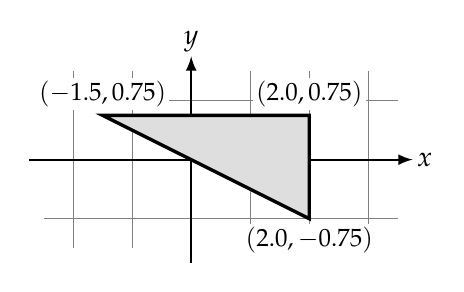
\begin{tikzpicture}[scale=0.75, every node/.style={inner sep=.25ex}]
	% \filldraw [white, draw=saitMaroon, thick, drop shadow={opacity=0.25}] (-0, 0) rectangle (3, 4);
	\coordinate (A) at (-1.5,0.75);
	\coordinate (B) at (2,-1);
	\coordinate (C) at (2,0.75);
	\draw[gray] (-2.5, -1.5) grid (3.5, 1.5);
	\draw [thick, black, -latex] (-2.75, 0) -- (3.75, 0) node[black, right] {$x$};
	\draw [thick, black, -latex] (0, -1.75) -- (0, 1.75) node[black, above] {$y$};
	\filldraw[very thick, fill=Gray0!50,draw=black] (A) -- (B) -- (C) -- cycle;
	\node[above = 0.35ex, fill=white] at (A) {\small $\left(-1.5, 0.75 \right)$};
	\node[below = 0.35ex, fill=white] at (B) {\small $\left(2.0, -0.75 \right)$};
	\node[above = 0.35ex, fill=white] at (C) {\small $\left(2.0, 0.75 \right)$};

\end{tikzpicture}

	}
\end{textblock*}


\begin{textblock*}{3in}(1in, 2in)
	\large
	\begin{align*}
		\overline{x} &= (2.0)-\frac{2.0-(-1.5)}{3}=0.83333 \\[0.25em]
		\overline{y} &= (0.75)-\frac{0.75-(-0.75)}{3}=0.25000		
	\end{align*}
	\par
	$$ \bm{\left(\overline{x},\overline{y}\right) = (0.83, 0.25)} $$
\end{textblock*}



\begin{textblock*}{3in}(1in, 3.75in)
	\cbox{
		Exercise 2: Determine the coordinates of the centroid of the semi-circle shown.
	}
\end{textblock*}
\begin{textblock*}{3.25in}(4.525in, 3.75in)
	\cbox{
		\centering
		\def\scale{1}
		% !TEX root = ../all/statikz.tex

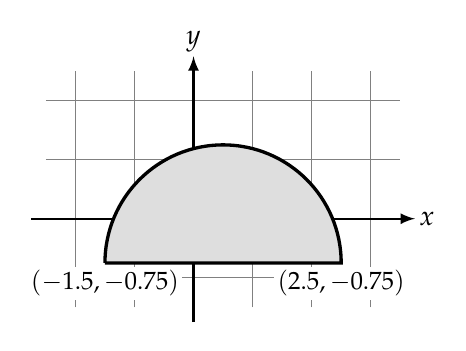
\begin{tikzpicture}[scale=0.75, every node/.style={inner sep=.25ex}]
  % \filldraw [white, draw=saitMaroon, thick, drop shadow={opacity=0.25}] (-0, 0) rectangle (3, 4);
  \coordinate (A) at (-1.5,-0.75);
  \coordinate (B) at (2.5,-0.75);
  \draw[gray] (-2.5, -1.5) grid (3.5, 2.5);
  \draw [thick, black,-latex] (-2.75, 0) -- (3.75, 0) node[black, right] {$x$};
  \draw [thick, black,-latex] (0, -1.75) -- (0, 2.75) node[black, above] {$y$};
  \filldraw[very thick, fill=Gray0!50,draw=black] (A) -- (B) arc (0:180:2cm);
  \node[below = 0.275ex, fill=white] at (A) {\small $\left(-1.5, -0.75\right)$};
  \node[below = 0.275ex, fill=white] at (B) {\small $\left(2.5, -0.75\right)$};

\end{tikzpicture}

	}
\end{textblock*}
\begin{textblock*}{3in}(1in, 4.875in)
	\large
	\begin{align*}
		r &= 2.0 \\[0.25em]
		\overline{x} &= \frac{(-1.5)+(2.5)}{2}=0.50 \\[0.25em]
		\overline{y} &= -0.75+\frac{4\x2.0}{3\pi}=0.098826
	\end{align*}
	\par
	$$ \bm{\left(\overline{x},\overline{y}\right) = (0.50, 0.99)} $$
\end{textblock*}

\begin{textblock*}{3in}(1in, 7in)
	\cbox{
			Exercise 3: Determine the location of the centroid of the quarter-circle shown.
	}
\end{textblock*}
\begin{textblock*}{3.25in}(4.525in, 7in)
	\cbox{
		\centering
		\def\scale{1}
		% !TEX root = ../all/statikz.tex

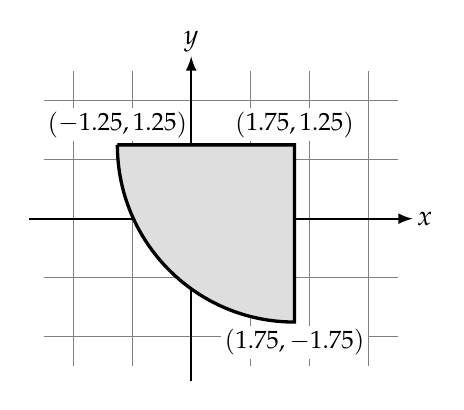
\begin{tikzpicture}[scale=0.75, every node/.style={inner sep=.25ex}]
	% \filldraw [white, draw=saitMaroon, thick, drop shadow={opacity=0.25}] (-0, 0) rectangle (3, 4);
	\coordinate (A) at (-1.25, 1.25);
	\coordinate (B) at (1.75,1.25);
	\coordinate (C) at (1.75,-1.75);
	\draw[gray] (-2.5, -2.5) grid (3.5, 2.5);
	\draw [thick, black, -latex] (-2.75, 0) -- (3.75, 0) node[black, right] {$x$};
	\draw [thick, black, -latex] (0, -2.75) -- (0, 2.75) node[black, above] {$y$};
	\filldraw[very thick, fill=Gray0!50,draw=black] (A) -- (B) -- (C) arc (270:180:3cm);
	\node[above = 0.275ex, fill=white] at (A) {\small $\left(-1.25, 1.25\right)$};
	\node[above = 0.275ex, fill=white] at (B) {\small $\left(1.75, 1.25\right)$};
	\node[below = 0.275ex, fill=white] at (C) {\small $\left(1.75, -1.75\right)$};

\end{tikzpicture}

	}
\end{textblock*}
\begin{textblock*}{3in}(1in, 8in)
	\large
	\begin{align*}
		r &= 3.00 \\[0.25em]
		\overline{x} &= 1.75-\frac{4\x3.00}{3\pi}=0.47676 \\[0.25em]
		\overline{y} &= 1.25-\frac{4\x3.00}{3\pi}=-0.023240
	\end{align*}
	\par
	$$ \bm{\left(\overline{x},\overline{y}\right) = (0.477, -0.0232)} $$
\end{textblock*}

%%%%%%%%%%%%%%%%%%%%%%%%%%%%%%%%%%%%%%%%%%%%%%%%%%%%%%%%%%%%%%%%%%%%%%%%%%%%%%%%%%%%%%%%%%%%%%%%%%%%
% page 2 
%%%%%%%%%%%%%%%%%%%%%%%%%%%%%%%%%%%%%%%%%%%%%%%%%%%%%%%%%%%%%%%%%%%%%%%%%%%%%%%%%%%%%%%%%%%%%%%%%%%%
~\newpage

\begin{textblock*}{2.25in}(1in, 0.125in)
	\cbox{
		Exercise 4\parm
		Find the location of the centroid, $C$, relative to the point~$O$.

	}
\end{textblock*}
\begin{textblock*}{4.125in}(3.775in, 0.125in)
	\cbox{
	\centering
	\def\scale{1}
	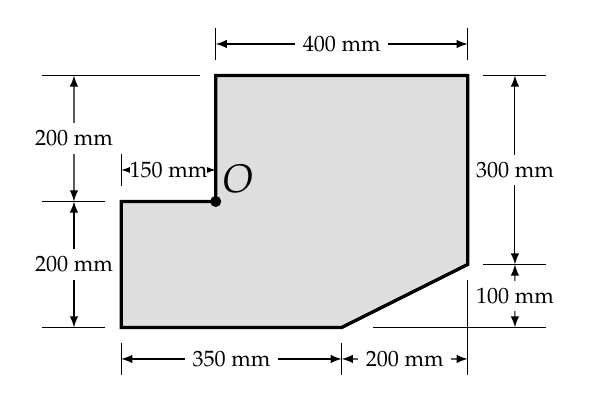
\begin{tikzpicture}[scale=0.8]

  \coordinate (O) at (0,0);
  \coordinate (B) at (0,2);
  \coordinate (C) at (4,2);
  \coordinate (D) at (4,-1);
  \coordinate (E) at (2,-2);
  \coordinate (F) at (-1.5,-2);
  \coordinate (G) at (-1.5,0);

  \draw ($ (B)+(0,0.25) $) -- +(0,.5);
  \draw ($ (C)+(0,0.25) $) -- +(0,.5);
  \draw ($ (G)+(0,0.25) $) -- +(0,0.5);

  \draw ($ (C)+(0.25, 0) $) -- +(1,0);
  \draw ($ (D)+(0.25, 0) $) -- +(1,0);
  \draw ($ (E)+(0.5, 0) $) -- +(2.75,0);

  \draw ($ (D)+(0, -0.25) $) -- +(0,-1.5);
  \draw ($ (E)+(0, -0.25) $) -- +(0,-.5);
  \draw ($ (F)+(0, -0.25) $) -- +(0,-.5);

  \draw ($ (F)+(-0.25, 0) $) -- +(-1,0);
  \draw ($ (G)+(-0.25, 0) $) -- +(-1,0);
  \draw ($ (B)+(-0.25, 0) $) -- +(-2.5,0);

  \footnotesize

  \draw[latex-latex] ($ (B)+(0,0.5) $) -- node[fill=white]{400 mm} ($ (C)+(0,0.5) $);
  \draw[latex-latex] ($ (G)+(0,0.5) $) -- node[fill=white, inner sep=0]{150 mm} ($ (O)+(0,0.5) $);
  \draw[latex-latex] ($ (D)-(0,1.5) $) -- node[fill=white]{200 mm} ($ (E)-(0,0.5) $);
  \draw[latex-latex] ($ (E)-(0,0.5) $) -- node[fill=white]{350 mm} ($ (F)-(0,0.5) $);
  \draw[latex-latex] ($ (C)+(0.75,0) $) -- node[fill=white]{300 mm} ($ (D)+(0.75,0) $);
  \draw[latex-latex] ($ (D)+(0.75,0) $) -- node[fill=white]{100 mm} ($ (E)+(2.75,0) $);
  \draw[latex-latex] ($ (F)-(0.75,0) $) -- node[fill=white]{200 mm} ($ (G)-(0.75,0) $);
  \draw[latex-latex] ($ (G)-(0.75,0) $) -- node[fill=white]{200 mm} ($ (B)-(2.25,0) $);


  \filldraw[draw=black, fill=Gray0!50, very thick] (O) -- (B) -- (C) -- (D) -- (E) -- (F) -- (G) -- cycle;
  \fill (O) circle (2.5pt);
  \footnotesize

  \node[above right, inner sep=0.1em, outer sep=0.25em] at (0,0) {\Large $O$};

\end{tikzpicture}

	}
\end{textblock*}

\begin{textblock*}{6.75in}(1in, 3in)
	\centering
	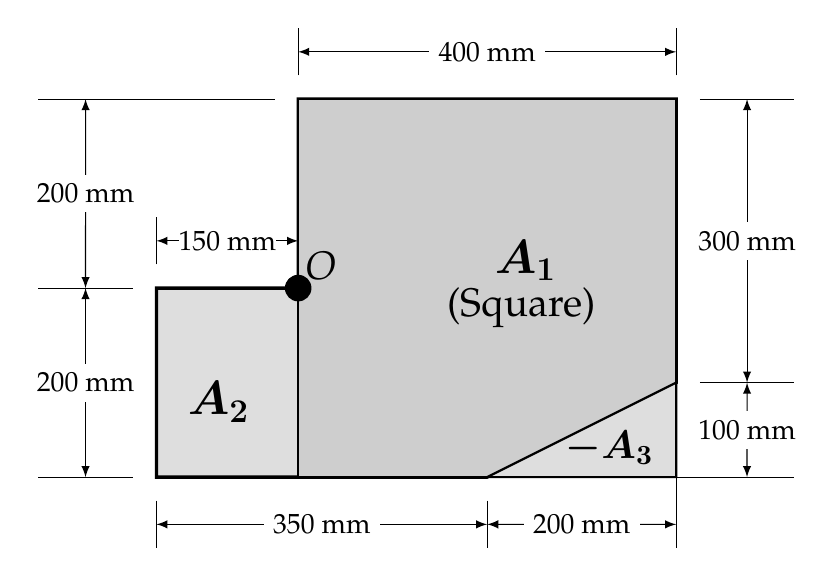
\begin{tikzpicture}[scale=1.2]

  \coordinate (O) at (0,0);
  \coordinate (B) at (0,2);
  \coordinate (C) at (4,2);
  \coordinate (D) at (4,-1);
  \coordinate (E) at (2,-2);
  \coordinate (F) at (-1.5,-2);
  \coordinate (G) at (-1.5,0);
  \coordinate (BR) at (4,-2);
  \coordinate (BO) at (0,-2);

  \draw ($ (B)+(0,0.25) $) -- +(0,.5);
  \draw ($ (C)+(0,0.25) $) -- +(0,.5);
  \draw ($ (G)+(0,0.25) $) -- +(0,0.5);

  \draw ($ (C)+(0.25, 0) $) -- +(1,0);
  \draw ($ (D)+(0.25, 0) $) -- +(1,0);
  \draw ($ (E)+(0.5, 0) $) -- +(2.75,0);

  \draw ($ (D)+(0, -0.25) $) -- +(0,-1.5);
  \draw ($ (E)+(0, -0.25) $) -- +(0,-.5);
  \draw ($ (F)+(0, -0.25) $) -- +(0,-.5);

  \draw ($ (F)+(-0.25, 0) $) -- +(-1,0);
  \draw ($ (G)+(-0.25, 0) $) -- +(-1,0);
  \draw ($ (B)+(-0.25, 0) $) -- +(-2.5,0);

  

  \draw[latex-latex] ($ (B)+(0,0.5) $) -- node[fill=white]{400 mm} ($ (C)+(0,0.5) $);
  \draw[latex-latex] ($ (G)+(0,0.5) $) -- node[fill=white, inner sep=0]{150 mm} ($ (O)+(0,0.5) $);
  \draw[latex-latex] ($ (D)-(0,1.5) $) -- node[fill=white]{200 mm} ($ (E)-(0,0.5) $);
  \draw[latex-latex] ($ (E)-(0,0.5) $) -- node[fill=white]{350 mm} ($ (F)-(0,0.5) $);
  \draw[latex-latex] ($ (C)+(0.75,0) $) -- node[fill=white]{300 mm} ($ (D)+(0.75,0) $);
  \draw[latex-latex] ($ (D)+(0.75,0) $) -- node[fill=white]{100 mm} ($ (E)+(2.75,0) $);
  \draw[latex-latex] ($ (F)-(0.75,0) $) -- node[fill=white]{200 mm} ($ (G)-(0.75,0) $);
  \draw[latex-latex] ($ (G)-(0.75,0) $) -- node[fill=white]{200 mm} ($ (B)-(2.25,0) $);


  \filldraw[draw=black, fill=Gray0!50, very thick] (O) -- (B) -- (C) -- (D) -- (E) -- (F) -- (G) -- cycle;
  

  \filldraw[fill=Gray0!75, thick] (O) -- (B) -- (C) -- (D) -- (BR) -- (E) -- (BO) -- cycle;
  \filldraw[fill=Gray0!50, thick] (D) -- (BR) -- (E)-- cycle;
  \footnotesize

  \node[above right, inner sep=0.1em, outer sep=0.25em] at (0,0) {\Large $O$};
  \node[above right, inner sep=0.1em, outer sep=0.25em] at (2,0) {\LARGE $\bm{A_1}$};
  \node[above right, inner sep=0.1em, outer sep=0.25em] at (1.5,-0.5) {\Large (Square)};
  \node[above right, inner sep=0.1em, outer sep=0.25em] at (-1.25,-1.5) {\LARGE $\bm{A_2}$};
  \node[above right, inner sep=0.1em, outer sep=0.25em] at (2.75,-1.95) {\Large $\bm{-A_3}$};

  \fill (O) circle (4pt);

\end{tikzpicture}

	\Large\parb\vspace{1cm}\centering
	\begin{tabular}{cccccc}
			Shape            & Area$\,\mathsf{\left(m^2 \right)}$                         & $x_i\,\mathsf{\left(m \right)}$               & $y_i\,\mathsf{\left(m \right)}$               & $A_ix_i\,\mathsf{\left(m^3 \right)}$                        & $A_iy_i\,\mathsf{\left(m^3 \right)}$                        \\
			\addlinespace
			\midrule
			$A_1$            & $0.4\x 0.4$                      & $0.2$            & $0$            & \textcolor{saitRed}{$0.032000$}   & \textcolor{saitRed}{$0$}   \\
			\midrule
			$A_2$            & $0.15\x0.2$                      & $-0.075$            & $-0.1$            & \textcolor{saitRed}{$-0.0022500$}   & \textcolor{saitRed}{$-0.0030000$}   \\
			\midrule
			$A_3$            & $-(0.2\x0.1)/2$                     & $0.33333$            & $-0.16667$           & \textcolor{saitRed}{$-0.0033333$}   & \textcolor{saitRed}{0.0016667}    \\
			
			\bottomrule\addlinespace
			{\Large$\Sigma$} & \textcolor{saitRed}{$0.18$} &                     &                     & \textcolor{saitRed}{$0.026417$}   & \textcolor{saitRed}{$-0.0013333$}
		\end{tabular}
		\parb
		\begin{align*}
			\overline{x} &= \frac{\sum A_ix_1}{\sum A_1}=\frac{0.026417}{0.18} = 0.14676\,\mathsf{m}\\\\
			\overline{y} &= \frac{\sum A_iy_1}{\sum A_1}=\frac{-0.0013333}{0.18} = -0.0074072\,\mathsf{m}
		\end{align*}
		\parb
		$$ \bm{(\overline{x}, \overline{y}) = (147\,\mathsf{mm}, -7.41\,\mathsf{mm})} $$
\end{textblock*}

%%%%%%%%%%%%%%%%%%%%%%%%%%%%%%%%%%%%%%%%%%%%%%%%%%%%%%%%%%%%%%%%%%%%%%%%%%%%%%%%%%%%%%%%%%%%%%%%%%%%
% page 4 
%%%%%%%%%%%%%%%%%%%%%%%%%%%%%%%%%%%%%%%%%%%%%%%%%%%%%%%%%%%%%%%%%%%%%%%%%%%%%%%%%%%%%%%%%%%%%%%%%%%%
~\newpage
% 

\begin{textblock*}{2.25in}(1in, 0.1in)
	\cbox{
		Exercise 5\parm
		Find the location of the centroid, $C$, relative to the coordinate origin.

	}
\end{textblock*}
\begin{textblock*}{4.125in}(3.775in, 0.1in)
	\cbox{
	\centering
	\def\scale{1}
	% !TEX root = ../all/statikz.tex

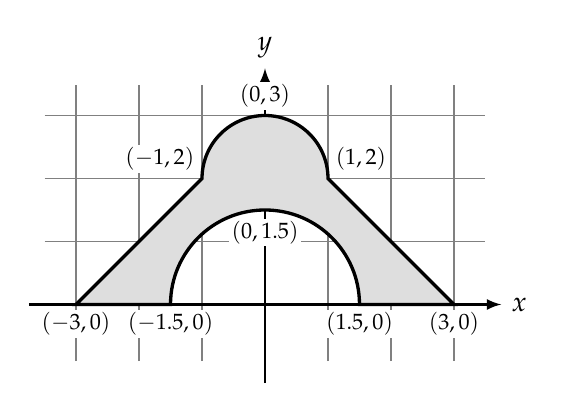
\begin{tikzpicture}[scale=0.8]
  \draw[gray] (-3.5,-.9) grid (3.5,3.49);
  \draw[-latex, thick, black] (-3.75, 0) -- (3.75, 0) node[right] {$x$};
  \draw[-latex, thick, black] (0, -1.25) -- (0,3.75) node[above] {$y$};
  \filldraw[draw=black, fill=Gray0!50, very thick] (-1.5,0) -- (-3, 0) -- (-1, 2) arc (180:0:1) -- (3,0)  -- (1.5,0) arc (0:180:1.5) -- cycle;
  \footnotesize

  \node[below, fill=white, inner sep=0.1em, outer sep=0.25em] at (-1.5,0) { $(-1.5, 0)$};
  \node[below, fill=white, inner sep=0.1em, outer sep=0.25em] at (-3,0) { $(-3, 0)$};
  \node[above left, fill=white, inner sep=0.1em, outer sep=0.25em] at (-1,2) { $(-1, 2)$};
  \node[above right, fill=white, inner sep=0.1em, outer sep=0.25em] at (1,2) { $(1, 2)$};
  \node[below, fill=white, inner sep=0.1em, outer sep=0.25em] at (3,0) { $(3, 0)$};
  \node[below, fill=white, inner sep=0.1em, outer sep=0.25em] at (1.5,0) { $(1.5, 0)$};
  \node[below, fill=white, inner sep=0.1em, outer sep=0.25em] at (0,1.45) { $(0, 1.5)$};
  \node[above, fill=white, inner sep=0.1em, outer sep=0.25em] at (0,3) { $(0,3)$};

\end{tikzpicture}

	}
\end{textblock*}

\begin{textblock*}{6.75in}(1in, 3in)
	\centering
	% !TEX root = ../all/statikz.tex

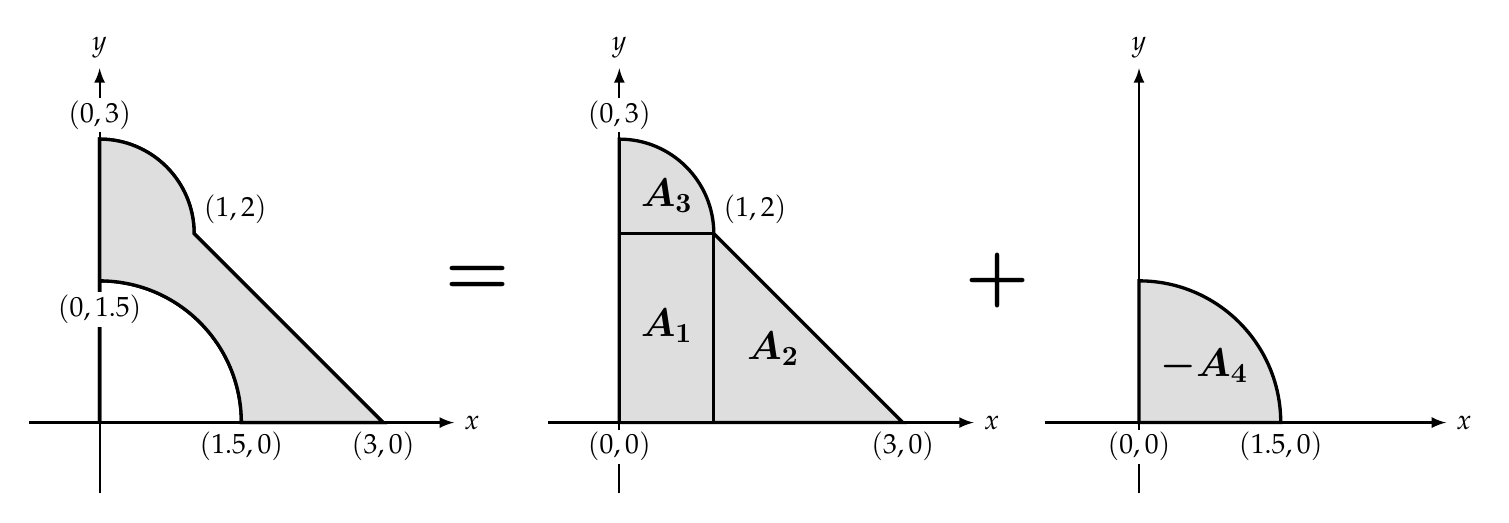
\begin{tikzpicture}[scale=1.2]
  \draw[-latex, thick, black] (-.75, 0) -- (3.75, 0) node[right] {$x$};
  \draw[-latex, thick, black] (0, -0.75) -- (0,3.75) node[above] {$y$};
  \filldraw[draw=black, fill=Gray0!50, very thick] (0,0) -- (0,3) arc (90:0:1) -- (3,0)  -- (1.5,0) arc (0:90:1.5) -- cycle;
  \node at (4,1.5) {\Huge$\bm =$};
  \node at (9.5,1.5) {\Huge$\bm +$};
  \draw[-latex, thick, black] (4.75, 0) -- (9.25, 0) node[right] {$x$};
  \draw[-latex, thick, black] (5.5, -0.75) -- (5.5,3.75) node[above] {$y$};
  \filldraw[draw=black, fill=Gray0!50, very thick] (0,0) -- (0,3) arc (90:0:1) -- (3,0)  -- (1.5,0) arc (0:90:1.5) -- cycle;
  \filldraw[draw=black, fill=Gray0!50, very thick] (5.5,0) -- (5.5,3) arc (90:0:1) -- (8.5,0)  -- (7,0)--(5.5,0) -- cycle;
  \filldraw[draw=black, fill=Gray0!50, very thick] (5.5,0) rectangle +(1,2);
  \draw[-latex, thick, black] (10, 0) -- (14.25, 0) node[right] {$x$};
  \draw[-latex, thick, black] (11, -0.75) -- (11,3.75) node[above] {$y$};
   \filldraw[draw=black, fill=Gray0!50, very thick] (11,0)--(11,1.5) arc (90:0:1.5) -- (11,0)  -- cycle;


  \node[above right, fill=white, inner sep=0.1em, outer sep=0.25em] at (1,2) { \normalsize $(1, 2)$};
  \node[below, fill=white, inner sep=0.1em, outer sep=0.25em] at (3,0) { \normalsize  $(3, 0)$};
  \node[below, fill=white, inner sep=0.1em, outer sep=0.25em] at (1.5,0) { \normalsize  $(1.5, 0)$};
  \node[below, fill=white, inner sep=0.1em, outer sep=0.25em] at (0,1.45) { \normalsize  $(0, 1.5)$};
  \node[above, fill=white, inner sep=0.1em, outer sep=0.25em] at (0,3) { \normalsize  $(0,3)$};
  \node[above right, fill=white, inner sep=0.1em, outer sep=0.25em] at (6.5,2) {  \normalsize $(1, 2)$};
  \node[below, fill=white, inner sep=0.1em, outer sep=0.25em] at (8.5,0) { \normalsize  $(3, 0)$};
  % \node[below, fill=white, inner sep=0.1em, outer sep=0.25em] at (7,0) { \normalsize  $(1.5, 0)$};
  \node[below, fill=white, inner sep=0.1em, outer sep=0.25em] at (5.5,0) { \normalsize  $(0, 0)$};
  \node[above, fill=white, inner sep=0.1em, outer sep=0.25em] at (5.5,3) { \normalsize  $(0,3)$};

  \node[above right, inner sep=0.1em, outer sep=0.25em] at (5.625,0.75) {\Large $\bm{A_1}$};
  \node[above right, inner sep=0.1em, outer sep=0.25em] at (6.75,0.5) {\Large $\bm{A_2}$};
  \node[above right, inner sep=0.1em, outer sep=0.25em] at (5.625,2.125) {\Large $\bm{A_3}$};
  \node[above right, inner sep=0.1em, outer sep=0.25em] at (11.125,0.325) {\Large $\bm{-A_4}$};
  \node[below, fill=white, inner sep=0.1em, outer sep=0.25em] at (11,0) { \normalsize  $(0, 0)$};
  \node[below, fill=white, inner sep=0.1em, outer sep=0.25em] at (12.5,0) { \normalsize  $(1.5, 0)$};
\end{tikzpicture}

	\Large\parb\vspace{1cm}\centering
	\begin{tabular}{cccc}
			Shape  & Area  & $y_i$ & $A_iy_i$   \\
			\addlinespace
			\midrule
			$A_1$  & $1\x 2$   & $1$  & \textcolor{saitRed}{$2$}   \\
			\midrule
			$A_2$  & $(2\x 2)/2$ & $0.66667$  & \textcolor{saitRed}{$1.3333$}   \\
			\midrule
			$A_3$  & $\pi/4$  & $2+\dfrac{4}{3\pi}$ & \textcolor{saitRed}{1.9041}    \\
			\midrule
			$-A_4$  & $-\dfrac{\pi(1.5)^2}{4}$  & $\dfrac{4\x 1.5}{3\pi}$ & \textcolor{saitRed}{-1.125}    \\
			
			\bottomrule\addlinespace
			{\Large$\Sigma$} & \textcolor{saitRed}{$3.0183$} &   & \textcolor{saitRed}{$4.1124$}
		\end{tabular}
		\parb
		\begin{align*}
			\overline{y} &= \frac{\sum A_iy_1}{\sum A_1}=\frac{4.1124}{3.0183} = 1.3625
		\end{align*}
		\parb
		$$ \bm{(\overline{x}, \overline{y}) = (0, 1.36)} $$
\end{textblock*}


%%%%%%%%%%%%%%%%%%%%%%%%%%%%%%%%%%%%%%%%%%%%%%%%%%%%%%%%%%%%%%%%%%%%%%%%%%%%%%%%%%%%%%%%%%%%%%%%%%%%
% page 4
%%%%%%%%%%%%%%%%%%%%%%%%%%%%%%%%%%%%%%%%%%%%%%%%%%%%%%%%%%%%%%%%%%%%%%%%%%%%%%%%%%%%%%%%%%%%%%%%%%%%
~\newpage


\begin{textblock*}{3.25in}(1in, 0.125in)
	\cbox{
		Exercise 6\parm
		Three C130X13 channels and a steel plate ($15\mathsf{mm}\x 174\mathsf{mm}$) are welded together. \parm
		Determine the location of the centroid, relative to the bottom left hand corner of the composite area.
		\ccbox[0.5]{white}{white}{
		Properties for C130X13:\pars
		Area $= 1700\,\mathsf{mm^2}$\lb
		Depth $=127\,\mathsf{mm}$\lb
		$\overline{x} =12\,\mathsf{mm}$\parb}
	}
\end{textblock*}
\begin{textblock*}{3in}(4.875in, 0.125in)
	\cbox{
	\centering
	\def\scale{0.65}
	% !TEX root = ../all/statikz.tex

\tikz{
  
  \def\fill{gray!50!white}
  \def\draw{gray!50!black}
  \begin{scope}[scale=\scale]
    \begin{scope}
      \filldraw[rounded corners=1pt,draw=gray!50!black, fill=gray!50!white, thick] (0,0) -- (2, 0) arc(0:85:0.25) -- (0.4,0.4) -- +(0, 5.2) -- (1.775,5.75)arc(-85:0:0.25) -- +(-2,0) -- cycle;
    \end{scope}

    \begin{scope}[yshift=6cm, xshift=6cm]
      \filldraw[rounded corners=1pt,draw=gray!50!black, rotate=180, fill=gray!50!white, thick] (0,0) -- (2, 0) arc(0:85:0.25) -- (0.4,0.4) -- +(0, 5.2) -- (1.775,5.75)arc(-85:0:0.25) -- +(-2,0) -- cycle;
    \end{scope}

    \begin{scope}[yshift=6cm, xshift=6cm]
      \filldraw[rounded corners=1pt,draw=gray!50!black, fill=gray!50!white, thick, rotate=90] (0,0) -- (2, 0) arc(0:85:0.25) -- (0.4,0.4) -- +(0, 5.2) -- (1.775,5.75)arc(-85:0:0.25) -- +(-2,0) -- cycle;
    \end{scope}

    \filldraw[rounded corners=1pt,draw=gray!50!black, fill=gray!50!white, thick] (-.5,0) rectangle (0,8);

    \node[below left] at (0,0) {$(0,0)$};
    \node at (-1.25,4) {\Large $A_4$};
    \node at (3,7) {\Large $A_1$};
    \node at (1.125,3) {\Large $A_2$};
    \node at (5,3) {\Large $A_3$};

  \end{scope}
}

	}
\end{textblock*}

\begin{textblock*}{6.5in}(1in,3in)
	\centering	
	\Large\parb\vspace{1cm}\centering
	\begin{tabular}{cccccc}
			Shape  & Area$ (\mathsf{mm^2})$  & $x_i\,\mathsf{(mm)}$ & $y_i\,\mathsf{(mm)}$ & $A_ix_i\,\mathsf{(mm^3)}$ & $A_iy_i\,\mathsf{ (mm^3)}$   \\
			\addlinespace
			\toprule\addlinespace
			$A_1$  & $1700$   & $15+\dfrac{127}{2}$  & $127+12$ & \textcolor{red}{133450} & \textcolor{red}{219300}  \\
			\addlinespace\midrule\addlinespace
			$A_2$  & $1700$ & $15+12$  & $\dfrac{127}{2}$ & \textcolor{red}{45900} & \textcolor{red}{107950}  \\
			\addlinespace\midrule\addlinespace
			$A_3$  & $1700$  & $15+127-12$ &  $\dfrac{127}{2}$  & \textcolor{red}{221000} & \textcolor{red}{107950}  \\
			\addlinespace\midrule\addlinespace
			$A_4$  & $2610$  & $7.5$ & $87$  & \textcolor{red}{19575} & \textcolor{red}{227070}  \\
			
			\addlinespace\bottomrule\addlinespace
			{$\sum$} & \textcolor{saitRed}{$7710$} &  & & \textcolor{saitRed}{$419925$} & \textcolor{saitRed}{$662270$}
		\end{tabular}
		\parb
		\begin{align*}
			\overline{x} &= \frac{\sum A_ix_1}{\sum A_1}=\frac{419925}{7710} = 54.465 \\\\
			\overline{y} &= \frac{\sum A_iy_1}{\sum A_1}=\frac{662270}{7710} = 85.898
		\end{align*}
		\parb
		$$ \bm{(\overline{x}, \overline{y}) = (54.5\,\mathsf{mm}, 85.9\,\mathsf{mm})} $$
\end{textblock*}



\end{document}